% Created by tikzDevice version 0.10.1 on 2016-08-29 22:50:31
% !TEX encoding = UTF-8 Unicode
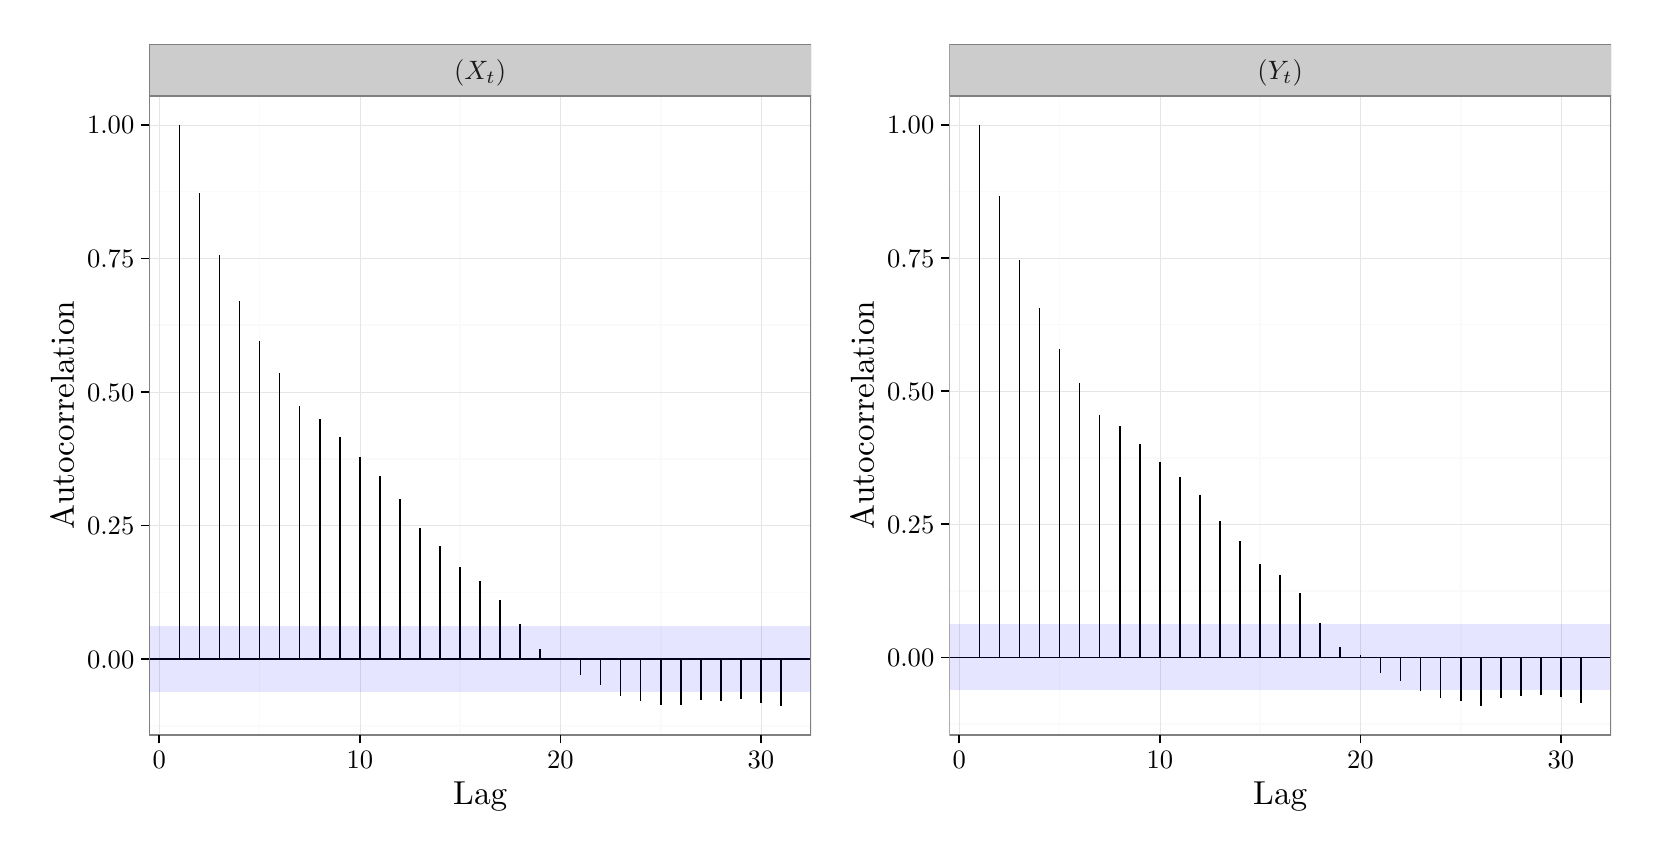
\begin{tikzpicture}[x=1pt,y=1pt]
\definecolor{fillColor}{RGB}{255,255,255}
\path[use as bounding box,fill=fillColor,fill opacity=0.00] (0,0) rectangle (578.16,289.08);
\begin{scope}
\path[clip] (  0.00,  0.00) rectangle (289.08,289.08);
\definecolor{drawColor}{RGB}{255,255,255}
\definecolor{fillColor}{RGB}{255,255,255}

\path[draw=drawColor,line width= 0.6pt,line join=round,line cap=round,fill=fillColor] (  0.00,  0.00) rectangle (289.08,289.08);
\end{scope}
\begin{scope}
\path[clip] ( 43.93, 33.48) rectangle (283.08,264.47);
\definecolor{fillColor}{RGB}{255,255,255}

\path[fill=fillColor] ( 43.93, 33.48) rectangle (283.08,264.47);
\definecolor{drawColor}{gray}{0.98}

\path[draw=drawColor,line width= 0.6pt,line join=round] ( 43.93, 36.73) --
	(283.08, 36.73);

\path[draw=drawColor,line width= 0.6pt,line join=round] ( 43.93, 85.01) --
	(283.08, 85.01);

\path[draw=drawColor,line width= 0.6pt,line join=round] ( 43.93,133.28) --
	(283.08,133.28);

\path[draw=drawColor,line width= 0.6pt,line join=round] ( 43.93,181.56) --
	(283.08,181.56);

\path[draw=drawColor,line width= 0.6pt,line join=round] ( 43.93,229.83) --
	(283.08,229.83);

\path[draw=drawColor,line width= 0.6pt,line join=round] ( 83.79, 33.48) --
	( 83.79,264.47);

\path[draw=drawColor,line width= 0.6pt,line join=round] (156.26, 33.48) --
	(156.26,264.47);

\path[draw=drawColor,line width= 0.6pt,line join=round] (228.73, 33.48) --
	(228.73,264.47);
\definecolor{drawColor}{gray}{0.90}

\path[draw=drawColor,line width= 0.2pt,line join=round] ( 43.93, 60.87) --
	(283.08, 60.87);

\path[draw=drawColor,line width= 0.2pt,line join=round] ( 43.93,109.15) --
	(283.08,109.15);

\path[draw=drawColor,line width= 0.2pt,line join=round] ( 43.93,157.42) --
	(283.08,157.42);

\path[draw=drawColor,line width= 0.2pt,line join=round] ( 43.93,205.69) --
	(283.08,205.69);

\path[draw=drawColor,line width= 0.2pt,line join=round] ( 43.93,253.97) --
	(283.08,253.97);

\path[draw=drawColor,line width= 0.2pt,line join=round] ( 47.55, 33.48) --
	( 47.55,264.47);

\path[draw=drawColor,line width= 0.2pt,line join=round] (120.02, 33.48) --
	(120.02,264.47);

\path[draw=drawColor,line width= 0.2pt,line join=round] (192.49, 33.48) --
	(192.49,264.47);

\path[draw=drawColor,line width= 0.2pt,line join=round] (264.96, 33.48) --
	(264.96,264.47);
\definecolor{drawColor}{RGB}{0,0,0}

\path[draw=drawColor,line width= 0.6pt,line join=round] ( 43.93, 60.87) -- (283.08, 60.87);

\path[draw=drawColor,line width= 0.6pt,line join=round] ( 54.80,253.97) -- ( 54.80, 60.87);

\path[draw=drawColor,line width= 0.6pt,line join=round] ( 62.04,229.19) -- ( 62.04, 60.87);

\path[draw=drawColor,line width= 0.6pt,line join=round] ( 69.29,206.81) -- ( 69.29, 60.87);

\path[draw=drawColor,line width= 0.6pt,line join=round] ( 76.54,190.18) -- ( 76.54, 60.87);

\path[draw=drawColor,line width= 0.6pt,line join=round] ( 83.79,175.88) -- ( 83.79, 60.87);

\path[draw=drawColor,line width= 0.6pt,line join=round] ( 91.03,164.42) -- ( 91.03, 60.87);

\path[draw=drawColor,line width= 0.6pt,line join=round] ( 98.28,152.24) -- ( 98.28, 60.87);

\path[draw=drawColor,line width= 0.6pt,line join=round] (105.53,147.57) -- (105.53, 60.87);

\path[draw=drawColor,line width= 0.6pt,line join=round] (112.77,141.18) -- (112.77, 60.87);

\path[draw=drawColor,line width= 0.6pt,line join=round] (120.02,134.00) -- (120.02, 60.87);

\path[draw=drawColor,line width= 0.6pt,line join=round] (127.27,127.05) -- (127.27, 60.87);

\path[draw=drawColor,line width= 0.6pt,line join=round] (134.52,118.75) -- (134.52, 60.87);

\path[draw=drawColor,line width= 0.6pt,line join=round] (141.76,108.31) -- (141.76, 60.87);

\path[draw=drawColor,line width= 0.6pt,line join=round] (149.01,101.69) -- (149.01, 60.87);

\path[draw=drawColor,line width= 0.6pt,line join=round] (156.26, 94.04) -- (156.26, 60.87);

\path[draw=drawColor,line width= 0.6pt,line join=round] (163.50, 89.23) -- (163.50, 60.87);

\path[draw=drawColor,line width= 0.6pt,line join=round] (170.75, 82.23) -- (170.75, 60.87);

\path[draw=drawColor,line width= 0.6pt,line join=round] (178.00, 73.42) -- (178.00, 60.87);

\path[draw=drawColor,line width= 0.6pt,line join=round] (185.24, 64.48) -- (185.24, 60.87);

\path[draw=drawColor,line width= 0.6pt,line join=round] (192.49, 60.68) -- (192.49, 60.87);

\path[draw=drawColor,line width= 0.6pt,line join=round] (199.74, 55.20) -- (199.74, 60.87);

\path[draw=drawColor,line width= 0.6pt,line join=round] (206.99, 51.59) -- (206.99, 60.87);

\path[draw=drawColor,line width= 0.6pt,line join=round] (214.23, 47.60) -- (214.23, 60.87);

\path[draw=drawColor,line width= 0.6pt,line join=round] (221.48, 45.62) -- (221.48, 60.87);

\path[draw=drawColor,line width= 0.6pt,line join=round] (228.73, 44.33) -- (228.73, 60.87);

\path[draw=drawColor,line width= 0.6pt,line join=round] (235.97, 44.19) -- (235.97, 60.87);

\path[draw=drawColor,line width= 0.6pt,line join=round] (243.22, 46.19) -- (243.22, 60.87);

\path[draw=drawColor,line width= 0.6pt,line join=round] (250.47, 45.76) -- (250.47, 60.87);

\path[draw=drawColor,line width= 0.6pt,line join=round] (257.72, 46.52) -- (257.72, 60.87);

\path[draw=drawColor,line width= 0.6pt,line join=round] (264.96, 44.96) -- (264.96, 60.87);

\path[draw=drawColor,line width= 0.6pt,line join=round] (272.21, 43.98) -- (272.21, 60.87);
\definecolor{fillColor}{RGB}{0,0,255}

\path[fill=fillColor,fill opacity=0.10] ( 43.93, 48.90) rectangle (283.08, 72.84);
\definecolor{drawColor}{gray}{0.50}

\path[draw=drawColor,line width= 0.6pt,line join=round,line cap=round] ( 43.93, 33.48) rectangle (283.08,264.47);
\end{scope}
\begin{scope}
\path[clip] ( 43.93,264.47) rectangle (283.08,283.08);
\definecolor{drawColor}{gray}{0.50}
\definecolor{fillColor}{gray}{0.80}

\path[draw=drawColor,line width= 0.2pt,line join=round,line cap=round,fill=fillColor] ( 43.93,264.47) rectangle (283.08,283.08);
\definecolor{drawColor}{gray}{0.10}

\node[text=drawColor,anchor=base,inner sep=0pt, outer sep=0pt, scale=  0.96] at (163.50,270.47) {$(X_t)$};
\end{scope}
\begin{scope}
\path[clip] (  0.00,  0.00) rectangle (578.16,289.08);
\definecolor{drawColor}{RGB}{0,0,0}

\node[text=drawColor,anchor=base east,inner sep=0pt, outer sep=0pt, scale=  0.96] at ( 38.53, 57.57) {0.00};

\node[text=drawColor,anchor=base east,inner sep=0pt, outer sep=0pt, scale=  0.96] at ( 38.53,105.84) {0.25};

\node[text=drawColor,anchor=base east,inner sep=0pt, outer sep=0pt, scale=  0.96] at ( 38.53,154.11) {0.50};

\node[text=drawColor,anchor=base east,inner sep=0pt, outer sep=0pt, scale=  0.96] at ( 38.53,202.39) {0.75};

\node[text=drawColor,anchor=base east,inner sep=0pt, outer sep=0pt, scale=  0.96] at ( 38.53,250.66) {1.00};
\end{scope}
\begin{scope}
\path[clip] (  0.00,  0.00) rectangle (578.16,289.08);
\definecolor{drawColor}{RGB}{0,0,0}

\path[draw=drawColor,line width= 0.6pt,line join=round] ( 40.93, 60.87) --
	( 43.93, 60.87);

\path[draw=drawColor,line width= 0.6pt,line join=round] ( 40.93,109.15) --
	( 43.93,109.15);

\path[draw=drawColor,line width= 0.6pt,line join=round] ( 40.93,157.42) --
	( 43.93,157.42);

\path[draw=drawColor,line width= 0.6pt,line join=round] ( 40.93,205.69) --
	( 43.93,205.69);

\path[draw=drawColor,line width= 0.6pt,line join=round] ( 40.93,253.97) --
	( 43.93,253.97);
\end{scope}
\begin{scope}
\path[clip] (  0.00,  0.00) rectangle (578.16,289.08);
\definecolor{drawColor}{RGB}{0,0,0}

\path[draw=drawColor,line width= 0.6pt,line join=round] ( 47.55, 30.48) --
	( 47.55, 33.48);

\path[draw=drawColor,line width= 0.6pt,line join=round] (120.02, 30.48) --
	(120.02, 33.48);

\path[draw=drawColor,line width= 0.6pt,line join=round] (192.49, 30.48) --
	(192.49, 33.48);

\path[draw=drawColor,line width= 0.6pt,line join=round] (264.96, 30.48) --
	(264.96, 33.48);
\end{scope}
\begin{scope}
\path[clip] (  0.00,  0.00) rectangle (578.16,289.08);
\definecolor{drawColor}{RGB}{0,0,0}

\node[text=drawColor,anchor=base,inner sep=0pt, outer sep=0pt, scale=  0.96] at ( 47.55, 21.46) {0};

\node[text=drawColor,anchor=base,inner sep=0pt, outer sep=0pt, scale=  0.96] at (120.02, 21.46) {10};

\node[text=drawColor,anchor=base,inner sep=0pt, outer sep=0pt, scale=  0.96] at (192.49, 21.46) {20};

\node[text=drawColor,anchor=base,inner sep=0pt, outer sep=0pt, scale=  0.96] at (264.96, 21.46) {30};
\end{scope}
\begin{scope}
\path[clip] (  0.00,  0.00) rectangle (578.16,289.08);
\definecolor{drawColor}{RGB}{0,0,0}

\node[text=drawColor,anchor=base,inner sep=0pt, outer sep=0pt, scale=  1.20] at (163.50,  8.40) {Lag};
\end{scope}
\begin{scope}
\path[clip] (  0.00,  0.00) rectangle (578.16,289.08);
\definecolor{drawColor}{RGB}{0,0,0}

\node[text=drawColor,rotate= 90.00,anchor=base,inner sep=0pt, outer sep=0pt, scale=  1.20] at ( 16.66,148.97) {Autocorrelation};
\end{scope}
\begin{scope}
\path[clip] (289.08,  0.00) rectangle (578.16,289.08);
\definecolor{drawColor}{RGB}{255,255,255}
\definecolor{fillColor}{RGB}{255,255,255}

\path[draw=drawColor,line width= 0.6pt,line join=round,line cap=round,fill=fillColor] (289.08,  0.00) rectangle (578.16,289.08);
\end{scope}
\begin{scope}
\path[clip] (333.01, 33.48) rectangle (572.16,264.47);
\definecolor{fillColor}{RGB}{255,255,255}

\path[fill=fillColor] (333.01, 33.48) rectangle (572.16,264.47);
\definecolor{drawColor}{gray}{0.98}

\path[draw=drawColor,line width= 0.6pt,line join=round] (333.01, 37.45) --
	(572.16, 37.45);

\path[draw=drawColor,line width= 0.6pt,line join=round] (333.01, 85.57) --
	(572.16, 85.57);

\path[draw=drawColor,line width= 0.6pt,line join=round] (333.01,133.68) --
	(572.16,133.68);

\path[draw=drawColor,line width= 0.6pt,line join=round] (333.01,181.80) --
	(572.16,181.80);

\path[draw=drawColor,line width= 0.6pt,line join=round] (333.01,229.91) --
	(572.16,229.91);

\path[draw=drawColor,line width= 0.6pt,line join=round] (372.87, 33.48) --
	(372.87,264.47);

\path[draw=drawColor,line width= 0.6pt,line join=round] (445.34, 33.48) --
	(445.34,264.47);

\path[draw=drawColor,line width= 0.6pt,line join=round] (517.81, 33.48) --
	(517.81,264.47);
\definecolor{drawColor}{gray}{0.90}

\path[draw=drawColor,line width= 0.2pt,line join=round] (333.01, 61.51) --
	(572.16, 61.51);

\path[draw=drawColor,line width= 0.2pt,line join=round] (333.01,109.62) --
	(572.16,109.62);

\path[draw=drawColor,line width= 0.2pt,line join=round] (333.01,157.74) --
	(572.16,157.74);

\path[draw=drawColor,line width= 0.2pt,line join=round] (333.01,205.85) --
	(572.16,205.85);

\path[draw=drawColor,line width= 0.2pt,line join=round] (333.01,253.97) --
	(572.16,253.97);

\path[draw=drawColor,line width= 0.2pt,line join=round] (336.63, 33.48) --
	(336.63,264.47);

\path[draw=drawColor,line width= 0.2pt,line join=round] (409.10, 33.48) --
	(409.10,264.47);

\path[draw=drawColor,line width= 0.2pt,line join=round] (481.57, 33.48) --
	(481.57,264.47);

\path[draw=drawColor,line width= 0.2pt,line join=round] (554.04, 33.48) --
	(554.04,264.47);
\definecolor{drawColor}{RGB}{0,0,0}

\path[draw=drawColor,line width= 0.6pt,line join=round] (333.01, 61.51) -- (572.16, 61.51);

\path[draw=drawColor,line width= 0.6pt,line join=round] (343.88,253.97) -- (343.88, 61.51);

\path[draw=drawColor,line width= 0.6pt,line join=round] (351.12,228.38) -- (351.12, 61.51);

\path[draw=drawColor,line width= 0.6pt,line join=round] (358.37,205.17) -- (358.37, 61.51);

\path[draw=drawColor,line width= 0.6pt,line join=round] (365.62,187.91) -- (365.62, 61.51);

\path[draw=drawColor,line width= 0.6pt,line join=round] (372.87,172.86) -- (372.87, 61.51);

\path[draw=drawColor,line width= 0.6pt,line join=round] (380.11,160.52) -- (380.11, 61.51);

\path[draw=drawColor,line width= 0.6pt,line join=round] (387.36,149.21) -- (387.36, 61.51);

\path[draw=drawColor,line width= 0.6pt,line join=round] (394.61,145.12) -- (394.61, 61.51);

\path[draw=drawColor,line width= 0.6pt,line join=round] (401.85,138.71) -- (401.85, 61.51);

\path[draw=drawColor,line width= 0.6pt,line join=round] (409.10,131.97) -- (409.10, 61.51);

\path[draw=drawColor,line width= 0.6pt,line join=round] (416.35,126.61) -- (416.35, 61.51);

\path[draw=drawColor,line width= 0.6pt,line join=round] (423.60,120.36) -- (423.60, 61.51);

\path[draw=drawColor,line width= 0.6pt,line join=round] (430.84,110.86) -- (430.84, 61.51);

\path[draw=drawColor,line width= 0.6pt,line join=round] (438.09,103.43) -- (438.09, 61.51);

\path[draw=drawColor,line width= 0.6pt,line join=round] (445.34, 95.31) -- (445.34, 61.51);

\path[draw=drawColor,line width= 0.6pt,line join=round] (452.58, 91.13) -- (452.58, 61.51);

\path[draw=drawColor,line width= 0.6pt,line join=round] (459.83, 84.73) -- (459.83, 61.51);

\path[draw=drawColor,line width= 0.6pt,line join=round] (467.08, 73.88) -- (467.08, 61.51);

\path[draw=drawColor,line width= 0.6pt,line join=round] (474.32, 65.33) -- (474.32, 61.51);

\path[draw=drawColor,line width= 0.6pt,line join=round] (481.57, 62.34) -- (481.57, 61.51);

\path[draw=drawColor,line width= 0.6pt,line join=round] (488.82, 55.97) -- (488.82, 61.51);

\path[draw=drawColor,line width= 0.6pt,line join=round] (496.07, 53.11) -- (496.07, 61.51);

\path[draw=drawColor,line width= 0.6pt,line join=round] (503.31, 49.21) -- (503.31, 61.51);

\path[draw=drawColor,line width= 0.6pt,line join=round] (510.56, 46.76) -- (510.56, 61.51);

\path[draw=drawColor,line width= 0.6pt,line join=round] (517.81, 45.69) -- (517.81, 61.51);

\path[draw=drawColor,line width= 0.6pt,line join=round] (525.05, 43.98) -- (525.05, 61.51);

\path[draw=drawColor,line width= 0.6pt,line join=round] (532.30, 47.03) -- (532.30, 61.51);

\path[draw=drawColor,line width= 0.6pt,line join=round] (539.55, 47.69) -- (539.55, 61.51);

\path[draw=drawColor,line width= 0.6pt,line join=round] (546.80, 47.96) -- (546.80, 61.51);

\path[draw=drawColor,line width= 0.6pt,line join=round] (554.04, 47.07) -- (554.04, 61.51);

\path[draw=drawColor,line width= 0.6pt,line join=round] (561.29, 44.97) -- (561.29, 61.51);
\definecolor{fillColor}{RGB}{0,0,255}

\path[fill=fillColor,fill opacity=0.10] (333.01, 49.58) rectangle (572.16, 73.44);
\definecolor{drawColor}{gray}{0.50}

\path[draw=drawColor,line width= 0.6pt,line join=round,line cap=round] (333.01, 33.48) rectangle (572.16,264.47);
\end{scope}
\begin{scope}
\path[clip] (333.01,264.47) rectangle (572.16,283.08);
\definecolor{drawColor}{gray}{0.50}
\definecolor{fillColor}{gray}{0.80}

\path[draw=drawColor,line width= 0.2pt,line join=round,line cap=round,fill=fillColor] (333.01,264.47) rectangle (572.16,283.08);
\definecolor{drawColor}{gray}{0.10}

\node[text=drawColor,anchor=base,inner sep=0pt, outer sep=0pt, scale=  0.96] at (452.58,270.47) {$(Y_t)$};
\end{scope}
\begin{scope}
\path[clip] (  0.00,  0.00) rectangle (578.16,289.08);
\definecolor{drawColor}{RGB}{0,0,0}

\node[text=drawColor,anchor=base east,inner sep=0pt, outer sep=0pt, scale=  0.96] at (327.61, 58.20) {0.00};

\node[text=drawColor,anchor=base east,inner sep=0pt, outer sep=0pt, scale=  0.96] at (327.61,106.32) {0.25};

\node[text=drawColor,anchor=base east,inner sep=0pt, outer sep=0pt, scale=  0.96] at (327.61,154.43) {0.50};

\node[text=drawColor,anchor=base east,inner sep=0pt, outer sep=0pt, scale=  0.96] at (327.61,202.55) {0.75};

\node[text=drawColor,anchor=base east,inner sep=0pt, outer sep=0pt, scale=  0.96] at (327.61,250.66) {1.00};
\end{scope}
\begin{scope}
\path[clip] (  0.00,  0.00) rectangle (578.16,289.08);
\definecolor{drawColor}{RGB}{0,0,0}

\path[draw=drawColor,line width= 0.6pt,line join=round] (330.01, 61.51) --
	(333.01, 61.51);

\path[draw=drawColor,line width= 0.6pt,line join=round] (330.01,109.62) --
	(333.01,109.62);

\path[draw=drawColor,line width= 0.6pt,line join=round] (330.01,157.74) --
	(333.01,157.74);

\path[draw=drawColor,line width= 0.6pt,line join=round] (330.01,205.85) --
	(333.01,205.85);

\path[draw=drawColor,line width= 0.6pt,line join=round] (330.01,253.97) --
	(333.01,253.97);
\end{scope}
\begin{scope}
\path[clip] (  0.00,  0.00) rectangle (578.16,289.08);
\definecolor{drawColor}{RGB}{0,0,0}

\path[draw=drawColor,line width= 0.6pt,line join=round] (336.63, 30.48) --
	(336.63, 33.48);

\path[draw=drawColor,line width= 0.6pt,line join=round] (409.10, 30.48) --
	(409.10, 33.48);

\path[draw=drawColor,line width= 0.6pt,line join=round] (481.57, 30.48) --
	(481.57, 33.48);

\path[draw=drawColor,line width= 0.6pt,line join=round] (554.04, 30.48) --
	(554.04, 33.48);
\end{scope}
\begin{scope}
\path[clip] (  0.00,  0.00) rectangle (578.16,289.08);
\definecolor{drawColor}{RGB}{0,0,0}

\node[text=drawColor,anchor=base,inner sep=0pt, outer sep=0pt, scale=  0.96] at (336.63, 21.46) {0};

\node[text=drawColor,anchor=base,inner sep=0pt, outer sep=0pt, scale=  0.96] at (409.10, 21.46) {10};

\node[text=drawColor,anchor=base,inner sep=0pt, outer sep=0pt, scale=  0.96] at (481.57, 21.46) {20};

\node[text=drawColor,anchor=base,inner sep=0pt, outer sep=0pt, scale=  0.96] at (554.04, 21.46) {30};
\end{scope}
\begin{scope}
\path[clip] (  0.00,  0.00) rectangle (578.16,289.08);
\definecolor{drawColor}{RGB}{0,0,0}

\node[text=drawColor,anchor=base,inner sep=0pt, outer sep=0pt, scale=  1.20] at (452.58,  8.40) {Lag};
\end{scope}
\begin{scope}
\path[clip] (  0.00,  0.00) rectangle (578.16,289.08);
\definecolor{drawColor}{RGB}{0,0,0}

\node[text=drawColor,rotate= 90.00,anchor=base,inner sep=0pt, outer sep=0pt, scale=  1.20] at (305.74,148.97) {Autocorrelation};
\end{scope}
\end{tikzpicture}
